\documentclass[11pt,preprint]{aastex}

 \begin{document}

\title{VNC - Virtual Network Computing---\today}



\section{What is VNC}  
VNC provides a means to connect to a desktop environment on a remote computer over a network, translating keyboard strokes and mouse movements 
such that it is as if you were sitting physically at the computer's monitor.  If you want the full treatment, check out the Wikipedia article on the subject at \verb$http://en.wikipedia.org/wiki/Vnc$.  

\subsection{Terminology}
\begin{itemize}
\item {\bf VNC Server}: the software program or process running on a remote computer, to which you will connect.
\item {\bf VNC Client}: the software program running on your local computer, perhaps your laptop, that you will use to connect to the VNC server.
\item {\bf VNC Session}: a specfic instance of the VNC server.
\item {\bf SSH Server}: the secure shell server, the software program running on a remote computer that provides secure (encrypted) terminal access.
\item {\bf SSH Client}: the secure shell client, the software program running on your local computer that provides a means of connecting to a remote SSH server.
\end{itemize}
\subsection{Why is VNC Useful?}
Lots of reasons, many of which you will discover as you more frequently use remote unix servers for your research.  Some of the more important features are:
 \begin{itemize}
\item VNC sessions are persistent.  This means that they will continue to run even when you are not connected to them with a VNC client.  Practically speaking, 
suppose you connect to a VNC server using one of the computers in the Undergraduate Radio Astronomy Lab, launch IDL and begin writing some code or running a 
computation process.  Although you are an incredibly dedicated astronomy student, after awhile you decide that you'd like to go over to your significant other's house
and raid his/her fridge (and maybe get a little work done on the side).  But your IDL process is running, and you already have all these windows open and an environment set up!
VNC to the rescue!  Simply quit the VNC client program, logout of your computer and head out on your way.  When you get to your destination, open up your laptop, make a sandwich and
connect back to your VNC session.  Voil\'{a}!  Everything is exactly how you left it in the lab, IDL still crunching away. 

\item VNC sessions run in the background on remote servers.  This means that your VNC session will be essentially invisible to someone
else physically using the computer (at 'console').  You won't disturb them and they won't disturb you (unless they power down the computer). 

\item VNC sessions are reasonably safe and secure, when used as described here, and avoid many of the headaches associated with X11 tunneling.
\end{itemize}

\section{How does VNC work?}
Quite simply.  Consider two computers connected via a closed TCP/IP network, the Undergraduate Astronomy Lab LAN for example.  Let's call one of these computers
\verb$leo$ and the other \verb$vega$.  Let's suppose you would like to connect to a remote desktop on \verb$leo$ from \verb$vega$.  How would you do this with VNC?
\begin{enumerate}
\item Instantiate a VNC server on \verb$leo$.
\item Instantiate a VNC client on \verb$vega$, enter the address for \verb$leo$ and connect.
\end{enumerate}

This example is a little trivial though.  What you would *really* like to do is be able to connect to \verb$leo$ from home... or maybe while on vacation... in the Carribean, with an
ice cold Cruzan Single Barrel Mojito and.... well, nevermind, you get the idea.  But what's so complicated about that?  Just fire up the VNC client and enter the address
of the computer you want to connect to, right?  Unfortunately, no.  While VNC is incredibly useful, when used alone it isn't very secure.  Because of these security considerations, most
networked computers are configured to disallow inbound connections to local VNC servers coming from random computers on the internet.  In addition, as is the case in the Undergraduate Astronomy Lab, often computer networks have firewalls or gateways that seperate the computers you actually want to connect to (like \verb$leo$) from the internet.  When certain types of firewalls or 
gateways are in place, it is necessary to connect first to the gateway and then connect to your final destination.  You are probably already familiar with situations like this
if you have tried to remotely login to computers is the Undergraduate Astronomy Lab.

The solution? - SSH, or more precisely, SSH tunneling.

\section {What is SSH Tunneling?}
Just like a physical tunnel going under the ground protects you from customs agents while you are smuggling contraband out of Mexico into Arizona, an SSH tunnel protects your
unencrypted, unsecure VNC connection from eavesdroppers, hackers, crackers and phone phreaks.  You have probably used SSH to connect remotely to a shell on another computer, and 
maybe you have also used SSH to perform 'X11 Tunneling,' or passing X11 information from a remote computer back to yours.  What you might not know is that SSH connections
are encrypted, and that you can use these encrypted connections to pass any kind of information between networked computers, including VNC network traffic.  Thus, when we combine SSH
with VNC, we can securely access a remote desktop on any internet-connected computer in the world.

When you instantiate a VNC server, a TCP port is configured to accept incoming connections from VNC clients.  Usually this port is only accessible from the local host or other 
computers on the same subnet, behind the network's gateway or firewall.  An SSH tunnel works by binding a TCP port on your local machine, usually the same port as you want
to connect to on a remote machine, and seamlessly transfering data sent to your local machine on that port, through an SSH connection, to the port on the remote machine.  As far as the remote machine
is concerned, it appears as though you are actually connecting from \verb$localhost$, and thus allows the connection to take place.  As will be illustrated below, sometimes you want to
connect \emph{through} a gateway to a port on another server attached to the gateway.  An SSH tunnel can work here as well, but in this case the remote port isn't located on the host you SSH
into.  However, as long as the internal server will allow connections to the desired port \emph{from the gateway}, the SSH tunnel will function identically.
          

\section{Dependencies}

In order to use VNC in tunneling mode, four pieces of software are required:
\begin{enumerate}
\item An SSH server for the host computer (probably already exists).
\item A VNC server for the host computer (probably already exists).
\item An SSH client for the client computer.
\item A VNC client for the client computer.
\end{enumerate}
For our purposes we can disregard 1. and 2.  Here we will assume you are trying to connect to a VNC
server on a *nix computer with an Xvnc-like VNC installation and a properly functioning SSH server, such as any of the computers in the Undergraduate Astronomy Lab.

\subsection{Windows}
For an SSH client, I reccomend PuTTY: A Free Telnet SSH Client.  
It is available for download at \verb$http://www.chiark.greenend.org.uk/~sgtatham/putty/$.  Simply follow the installation
instructions provided on the download page.  It's available in multiple formats, but you will probably want 
this one: \verb$http://the.earth.li/~sgtatham/putty/latest/x86/putty.zip$.

For a VNC client, I would suggest TightVNC (also free).  It is available for download at \verb$http://www.tightvnc.com/$.  Installation instructions are
provided on the download page.  All you will probably need is the stable viewer executable.  The most recent version (at the time of this writing) is at: 
\verb$http://downloads.sourceforge.net/vnc-tight/tightvnc-1.3.10_x86_viewer.zip$.

\subsection{Linux, OSX and *nix}
Chances are very good that you already have an SSH client installed, try typing \verb$ssh$ on your command line.  If it appears you don't have an SSH client installed, refer to your OS installation media.

You might also have a VNC client installed already.  Try typing \verb$vncviewer$ on your command line.  If you are greeted with a blank stare by your shell, you will have to *eek* install a piece of software on a unix machine.  Don't worry, it's really not that 
bad.  I would suggest TightVNC, which is freely available at \verb$http://www.tightvnc.com$.  Binary distributions are available for most OSs, and source is provided 
for others.  You can also use your favorite package management tool (\verb$yum$, \verb$apt-get$, \verb$port$, \verb$fink$, etc...).  Try grep'ing a package list for \verb$vnc$ or \verb$Xvnc$.

\emph{Note for OSX:}\\
If you have trouble building TightVNC from source, or perhaps just prefer a pretty native GUI VNC client, you can try RealVNC, available at \verb$http://www.realvnc.com$
(download the free version) or Chicken of the VNC, available at \verb$http://sourceforge.net/projects/cotvnc/$.


\section{Basic Setup}

Let's first consider the simplest case.  Suppose you would like to setup a VNC server on an isolated computer (not behind a firewall), and connect to it
from your laptop via an SSH tunnel.  For this example, lets use the Undergraduate Astronomy Lab gateway, \verb$ugastro.berkeley.edu$ or \verb$aquarius$.  Note: You really
shouldn't run a VNC server (or IDL for that matter) on \verb$aquarius$, since it serves as the gateway for the rest of the lab.  Note: The server side of these instructions will implicitly assume that
the computer you want to connect to is Linux or *nix based, but VNC server software is available for just about any operating system.

\subsection{Starting the VNC Server}
\begin{enumerate}

\item Login to the remote machine \verb$ugastro.berkeley.edu$ using SSH.\\
\begin{verbatim}
**************************************************
Welcome to aquarius on the UGAstro network.

other "rack" computers: 
(vega, polaris, nemesis, europa)
***************************************************

asiemion@aquarius:~>
\end{verbatim}

\item Setup your VNC Desktop Environment.

VNC usually defaults to a plain, ugly and generally lame desktop environment.  You probably want something pretty, like what you see when you login at console.
Enter the commands:
\begin{verbatim}
asiemion@aquarius:~>mkdir ~/.vnc
asiemion@aquarius:~>vi ~/.vnc/xstartup
\end{verbatim}
Make sure your xstartup file looks like this: 
\begin{verbatim}
#!/bin/sh

unset SESSION_MANAGER
exec /etc/X11/xinit/xinitrc

[ -x /etc/vnc/xstartup ] && exec /etc/vnc/xstartup
[ -r $HOME/.Xresources ] && xrdb $HOME/.Xresources
xsetroot -solid grey
vncconfig -iconic &
xterm -geometry 80x24+10+10 -ls -title "$VNCDESKTOP Desktop" &
startx &
\end{verbatim}

\item Set your VNC password using the \verb$vncpasswd$ command.
\begin{verbatim}
asiemion@aquarius:~>vncpasswd
Using password file /home/asiemion/.vnc/passwd
Password: 
Warning: password truncated to the length of 8.
Verify:   
Would you like to enter a view-only password (y/n)? n
\end{verbatim}

You only have to do this once, and the password you enter will be used anytime you start a VNC server on the machine you logged into.  Make sure and choose a good password, 
your VNC password is just as important as your login password.  It's generally a good idea to use different passwords for your VNC session and login account.

\item Start the VNC Server
\begin{verbatim}
asiemion@aquarius:~>vncserver

Warning: aquarius:1 is taken because of /tmp/.X11-unix/X1
Remove this file if there is no X server aquarius:1

New 'X' desktop is aquarius:2

Starting applications specified in /home/asiemion/.vnc/xstartup
Log file is /home/asiemion/.vnc/aquarius:2.log
\end{verbatim}
What's with the warning, you ask?  All that means is that someone else (maybe you) is running a VNC server process using VNC desktop \verb$:1$.  The VNC server noticed this, and setup your 
server on desktop \verb$:2$.  Take note of the line \verb$New 'X' desktop is aquarius:2$.  This identifies the port that your VNC server will be operating on.  VNC port numbering begins at \verb$5900$ 
(for desktop \verb$:0$), continues to \verb$5901$ (for desktop \verb$:1$), then \verb$5902$ (for desktop \verb$:2$) and so on.
\end{enumerate}
\subsection {Configuring SSH and Logging in}
\subsubsection{Windows Instructions}
\begin{itemize}
\item Set up the SSH Tunnel
\begin{enumerate}
\item Launch PuTTY, Expand the \verb$SSH$ tab, and click on \verb$Tunnels$.  We saw earlier that the server was setup on desktop \verb$:2$, so we know the port
we want to connect to is \verb$5902$, and the host we want to connect to is \verb$localhost$ - i.e. the VNC server we want to connect to is \emph{running on} the machine
we are logging into.  Thus we enter \verb$localhost:5902$ in the \verb$Destination$ field - this represents where we want the tunnel to point to on the remote end.  To keep things easy to remember we enter the same port, \verb$5902$, in the \verb$Source port$ field - this represents where we want the tunnel to point on our end.
\\
\item Now click the \verb$Add$ button to confirm your entry and add it to the \verb$Forwarded ports:$ list.
\\
\\
As you can see, you have setup a tunnel from \verb$L5902$ (local port 5902) to \verb$localhost:5902$ (remote host port 5902).  Note that in the latter instance, 
\verb$localhost$ is referenced from the machine you are logging into.  On that machine \verb$ugastro.berkeley.edu$, \verb$localhost$ refers to itself, which is just what we want.
\\
\begin{figure}[h!]
\begin{center}
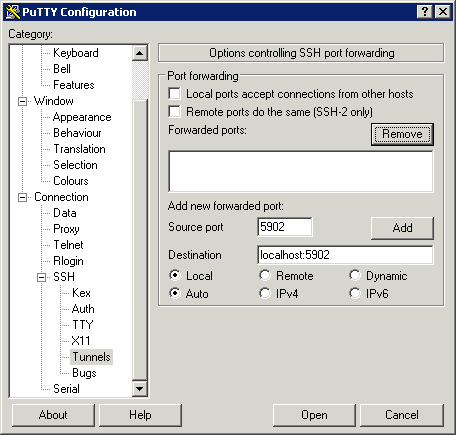
\includegraphics[scale=0.5]{putty1a.png}
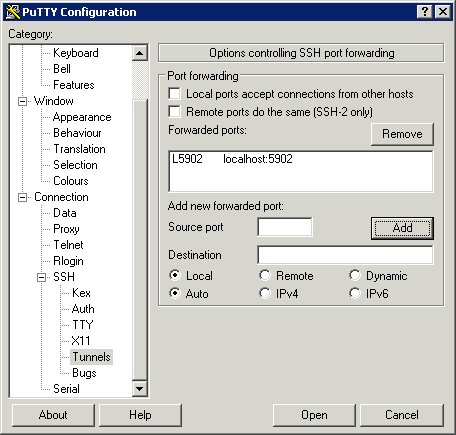
\includegraphics[scale=0.5]{putty2a.png}
\end{center}
\caption{Left: Step 1., Right: Step 2.}
\end{figure}
\\
\item Next click on the \verb$Session$ tab, and enter the name of the machine you want to login to, in this case \verb$ugastro.berkeley.edu$.

\begin{figure}[h!]
\begin{center}
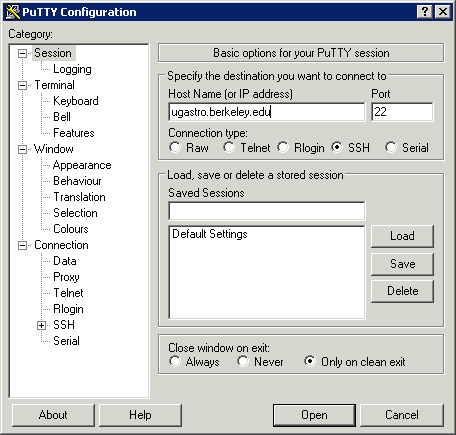
\includegraphics[scale=0.6]{putty3a.png}
\end{center}
\end{figure}

\item Click the \verb$Open$ button and login using your usual credentials.

\begin{figure}[h!]
\begin{center}
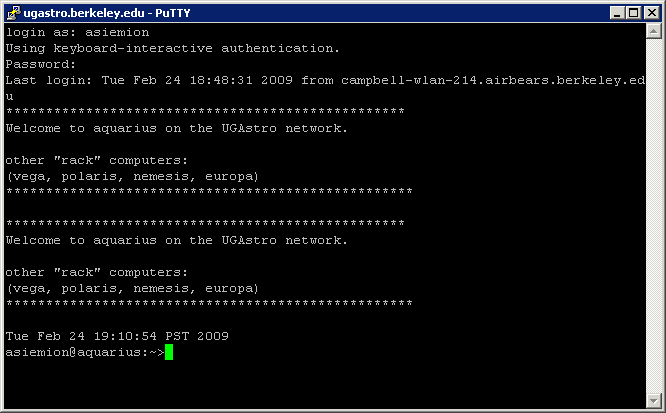
\includegraphics[scale=0.5]{putty4a.png}
\end{center}
\end{figure}

Don't close the window!  Just move it aside.  If you close this window, you will also close your SSH tunnel.
\end{enumerate}
\item Launch the VNC client and connect to the VNC session
\begin{enumerate}
\item Launch the VNC client, here we'll use TightVNC.  We know that we are using desktop \verb$:2$, so enter \verb$localhost:2$ in the \verb$VNC server:$ field.  Here, \verb$localhost$ refers to your own 
computer - SSH is \emph{tunneling} the remote host \verb$ugastro.berkeley.edu$'s port \verb$5902$ to your machine's port \verb$5902$.  Your VNC client knows that if you are asking for desktop \verb$:2$, this means port \verb$5902$.
\begin{figure}[h!]
\begin{center}
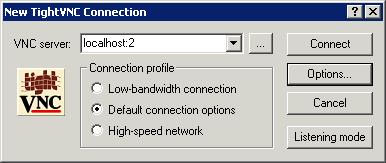
\includegraphics[scale=0.6]{putty5a.png}
\end{center}
\end{figure}
\item Click the connect button, and you will be asked for a password (as long as everything is working!)
%\begin{figure}[h!]
%\begin{center}
%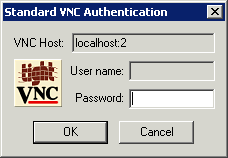
\includegraphics[scale=0.6]{putty6a.png}
%\end{center}
%\end{figure}
\\
\item Enter the VNC password you setup earlier.  If all goes well, you should see a desktop environment on the remote host.
\\
\begin{figure}[h!]
\begin{center}
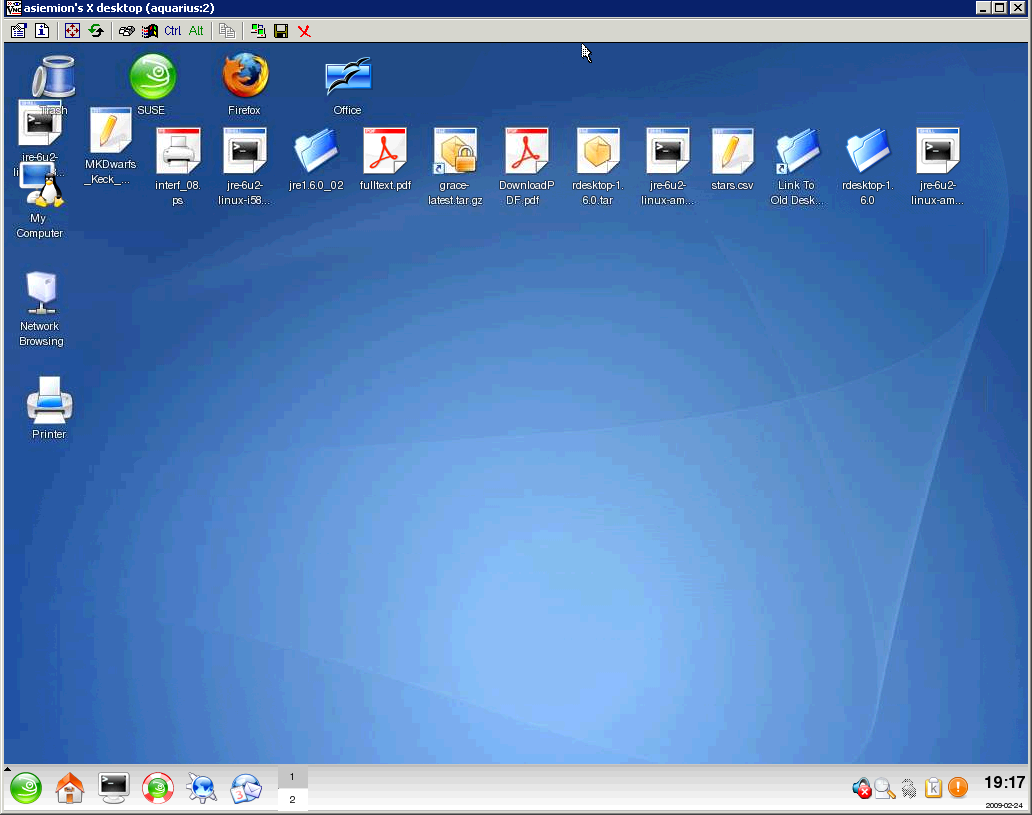
\includegraphics[scale=0.4]{putty7a.png}
\end{center}
\end{figure}
\end{enumerate}
\end{itemize}

\subsubsection{Linux, OS X and *nix Instructions}
\begin{itemize}
\item Set up the SSH Tunnel

Fire up your terminal and enter the following line:
\begin{verbatim}
$ ssh -L localhost:5902:localhost:5902 asiemion@ugastro.berkeley.edu -N -f
Password: 
\end{verbatim}
Enter your login password, and you should be returned to the command line.  

What does all that mean?  A little explanation is in order.  

The \verb$-L [bind_address:]port:host:hostport$ option to \verb$ssh$ instructs the SSH client to open a tunnel from \verb$bind_address:port$ to \verb$host:hostport$.  \verb$bind_address:port$
represents the local end of the tunnel, in this case we want the local end of the tunnel to be on port \verb$5902$ on our own computer, \verb$localhost$. 
We want the remote end of the tunnel, \verb$host:hostport$, to connect to port \verb$5902$ on the machine we are logging into, also called \verb$localhost$.  \verb$localhost$ can represent either 
the remote computer or the \emph{actual} local computer, depending on the context.  This can be a little confusing.  Try to remember that the computer reading the \verb$bind_address:port$
part is the local computer, and the computer reading the \verb$host:hostport$ part is the computer where you are connecting to.  Both computers consider themselves \verb$localhost$!  If you're 
still confused, read on.

The next argument specifies the login name and host we want to login to, \verb$user@host$.  The last two options tell SSH to go into the background after execution.

\item Launch the VNC client and connect to the VNC session

Enter the \verb$vncviewer$ command to connect to the VNC session.  Enter your previously-chosen VNC password when prompted.
\begin{verbatim}
$ vncviewer localhost:2
VNC viewer version 3.3.7 - built Feb 10 2009 17:36:02
Copyright (C) 2002-2003 RealVNC Ltd.
Copyright (C) 1994-2000 AT&T Laboratories Cambridge.
See http://www.realvnc.com for information on VNC.
VNC server supports protocol version 3.7 (viewer 3.3)
Password: 
VNC authentication succeeded
...
\end{verbatim}
For the host address we specified \verb$localhost:2$, since we terminated our SSH tunnel on our own machine (\verb$localhost$) port \verb$5902$.
\end{itemize}

\subsection{Closing Things Down}
\subsubsection{The Client Side}
Easy! Just close the windows.  Remember, terminating the VNC client doesn't affect the VNC server.  All your processes will continue to run, and your desktop will be just
as you left it when you log back in.  If you are using Linux or *nix, you will have to manually kill your SSH tunnel using the \verb$kill$ command.

\subsubsection{Terminating the VNC server}
\begin{enumerate}

\item Login to the remote machine \verb$ugastro.berkeley.edu$ using SSH.

\item Enter the \verb$vncserver$ command with the \verb$-kill$ option, followed by your desktop identifier, in this case desktop \verb$:2$.

\begin{verbatim}
asiemion@aquarius:~>vncserver -kill :2
Killing Xvnc process ID 31150
\end{verbatim}

\end{enumerate}

\section{Tunneling through a Gateway to a Remote Computer}

As mentioned earlier, sometimes you don't want to run the VNC server on the same machine you SSH into, like in the Undergraduate Astronomy Lab.  Can you still use an SSH tunnel in such a case?  Yes!  Remember, however, that you need to make sure the \emph{gateway} machine can connect to the \emph{destination} machine directly.  You can check if this is possible
by attempting to \verb$telnet$ from the gateway machine into the destination machine, on the port the VNC server is running on (see \verb$man telnet$).  If you can connect, you're in business.
\\

If you try the \verb$telnet$ trick and can't connect, you can still setup an SSH tunnel, albeit with a bit
more effort, but you might not want to - its liable to be pretty slow.  No need to check this for the Undergraduate Astronomy Lab though, the instructions below will work fine.

\subsection{Starting the VNC Server}

Follow the same procedure as above, but execute the commands on the machine where you want the VNC server to be running.  In keeping with our earlier examples, we'll setup the 
server on the Undergraduate Astronomy Lab machine \verb$leo$.

\begin{verbatim}
asiemion@leo:~>vncserver

New 'X' desktop is leo:1

Starting applications specified in /home/asiemion/.vnc/xstartup
Log file is /home/asiemion/.vnc/leo:1.log
\end{verbatim}

\subsection{Configuring SSH and Logging In}

Most of the instructions above apply to the gateway - remote computer situation as well, with one important exception.  In this case, the SSH tunnel needs to terminate at port \verb$5901$ on the machine \verb$leo$.  
We know this from looking at the output of the \verb$vncserver$ command, and noting that our desktop is on \verb$leo:1$.  Remember, the computer connecting to \verb$leo$ will be the \emph{gateway} we ssh into.  Its important
to use a machine name recognizable to the gateway when specifying the destination end of the SSH tunnel.  If you tried the \verb$telnet$ trick above, you already know whether or not you are using the correct machine name.

\pagebreak

\noindent For Windows, our SSH tunnel dialog would look like:

\begin{figure}[h!]
\begin{center}
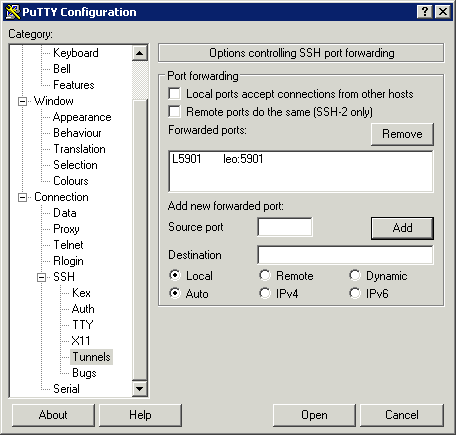
\includegraphics[scale=0.6]{putty3.png}
\end{center}
\end{figure}

\noindent In Linux, OSX or *nix, our SSH command would change to:
\begin{verbatim}
$ ssh -L localhost:5901:leo:5901 asiemion@ugastro.berkeley.edu -N -f
\end{verbatim}

As you can see, we are instructing the gateway machine, \verb$ugastro.berkeley.edu$ to terminate our tunnel at the internal host \verb$leo$ on port \verb$5901$.  Other settings should stay the same, 
except this time we would instruct our VNC client to connect to \verb$localhost:1$.  Desktop \verb$:1$ corresponds to port \verb$5901$.

\section{Final Thoughts}
\noindent Is that it?
\\
Not by a long shot.  There are all kinds of cool things you can do with SSH tunnels, and you will undoubtedly find myriads of uses for them as you continue your studies.  VNC has all kinds of cool applications as well.  GoToMyPC has made millions of dollars off of it!
\\
\\
One important VNC capability you should know about:
\\
VNC servers can have more than one VNC client connected to them, making VNC great for remote collaboration or just a rousing fight for control of the mouse. One can even setup a 'view only password' for VNC sessions, so that some participants can watch the screen without disturbing others.  Want to know how to set this up?  Just explore a bit and try a little trial and error!


\end{document}

















